
\documentclass{article}
\usepackage{graphicx}
\usepackage{amsmath}

\title{\textbf{The CT: Computational Text-Mining, Scholastic Capture, and the Flattening of the Indian Martial Body}}

\author{%
  \small Patrick S. D. MacCartney (Research Fellow), Anthropological Institute, Nanzan University, Japan;\\
  \small School of Culture, History and Language, Australian National University, Australia; Center for Regional Studies,\\
  \small Manipal Academy of Higher Education, India. Email: \texttt{p9856537@anu.edu.au}\\
  \small \date{August 7, 2026}
}

\begin{document}

\maketitle

\begin{abstract}
This paper outlines the ``Contortionist Turn (CT),'' a materialist framework charting the top-down scholastic capture, sanitization, and flattening of volatile subaltern physical survival practices. By deploying a high-performance parallelized text-mining pipeline across 20,529 Sanskrit text nodes, we track how raw kinetic technologies—engineered by specialized outcaste labor guilds like the \textit{Ḍombas} and \textit{Vaṃśa-nartins} for frontier defense and intelligence systems—were systematically turned inward and repackaged into the passive, quietistic metaphysical spine (\textit{merudaṇḍa}) of institutionalized yoga.
\end{abstract}

\vspace{1.5cm}

\clearpage 

\begin{figure}[p]
 \centering
 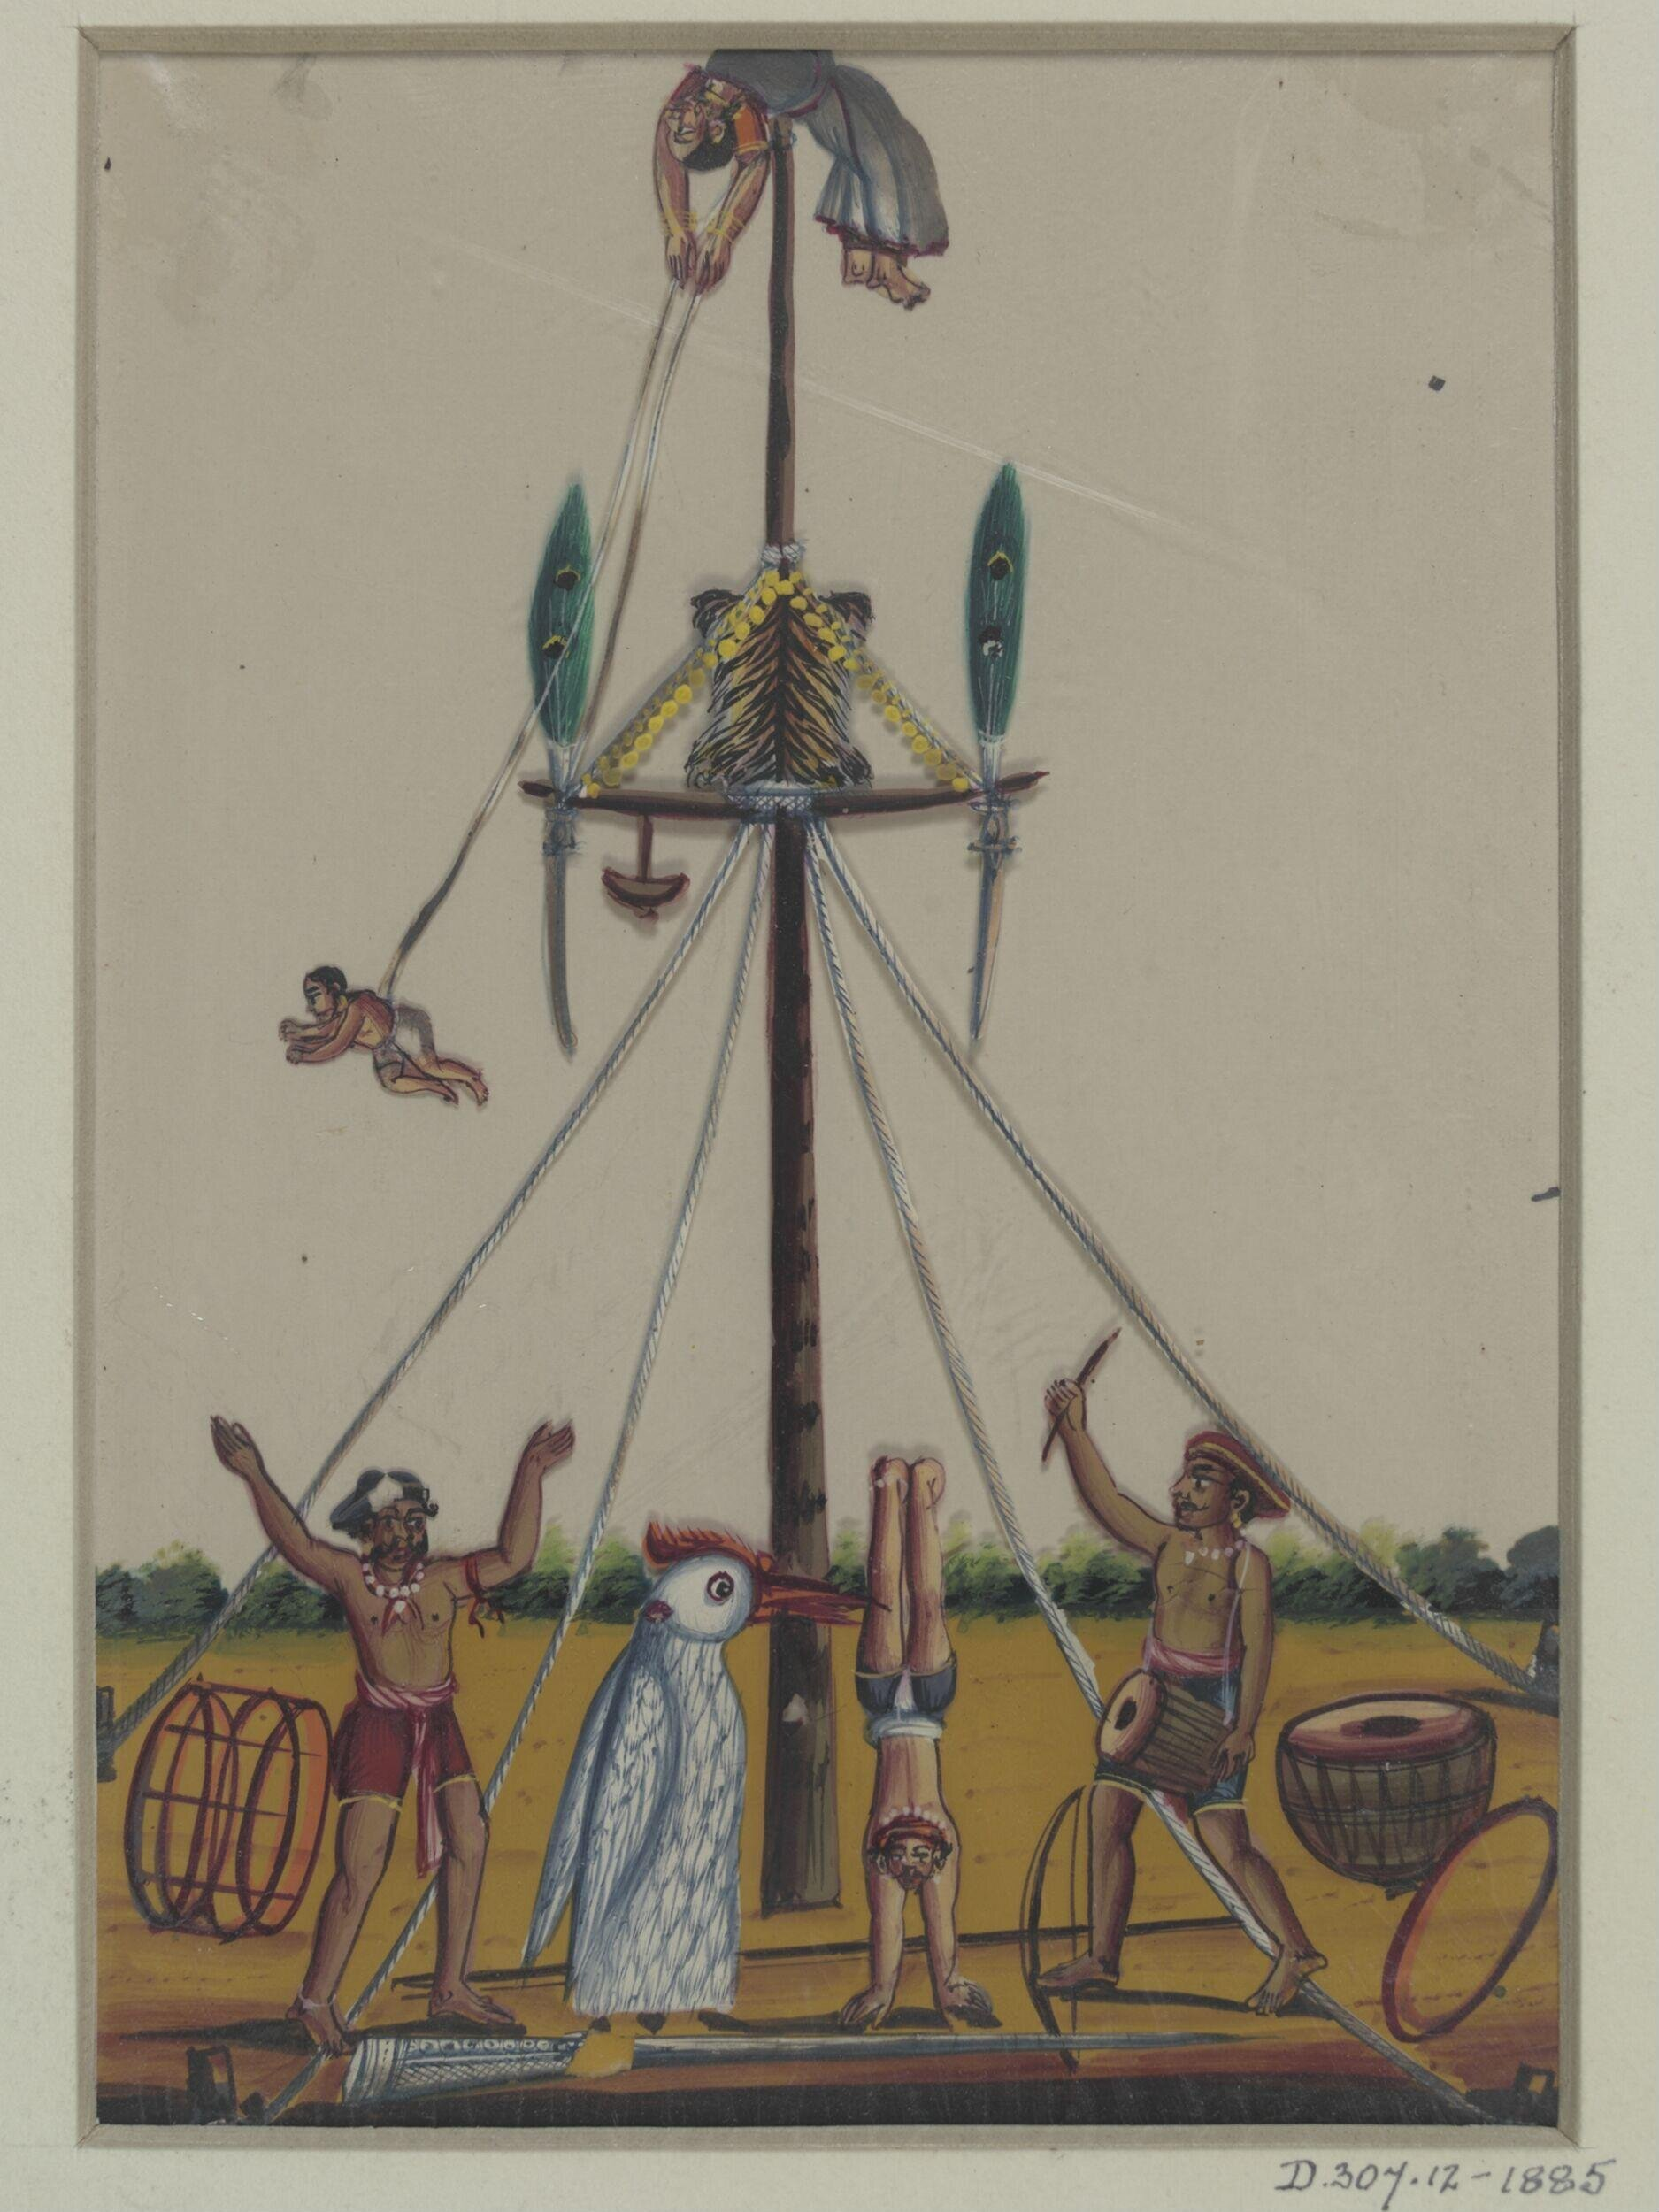
\includegraphics[width=0.75\textwidth]{kamatchiamma.jpg}
 \caption[Mid-nineteenth-century gouache on mica depicting Trichinopoly acrobat performances.]{Mid-nineteenth-century gouache on mica depicting Trichinopoly acrobat performances, showing vertical pole-balancing and suspended rope-somatic dynamics matching the historical \textit{upastambha} layout.}
 \label{fig:kamatchi_acrobats}
\end{figure}

\clearpage

\section{Introduction: The CT}
At the gates of the gopura of the Sri Kacchi Kāśmīra Avaṇiyā Temple in Kanchipuram, Tamil Nadu, a vertical bamboo pole measuring exactly seventy-two spans... This paradigm shifts what we call the CT into active empirical tracking.

\section{Conclusion}
Ultimately, the Contortionist Turn represents a massive paradigm shift. As the CT settles into mainstream scholarship, we must ensure its roots are remembered.
\end{document}
